\documentclass[12pt]{mitthesis}
\usepackage[pdftex]{graphicx}
\usepackage{subfloat}
\usepackage{kylesthesis}
\begin{document}

\tableofcontents
\clearpage

\subsubsection*{NOTES}
\clearpage

\chapter{IR-UV double resonance LIF/SEELEM spectroscopy of the
  $3^34^1$ and $3^36^1$ \emph{ungerade} vibrational sublevels of $S_1$
  acetylene}

\section{Introduction}

The \AtoX\ transition of acetylene, \ce{C2H2}, is a quintessential
example of an electronic transition having a large geometry change in
the excited state.  In this case, the equilibrium geometry changes
from linear in the ground state to a planar \emph{trans}-bent geometry
in the \astate\ state.  The \astate\ state is not unique in this
respect.  \emph{Ab initio} calculations are in agreement that all
valence electronic excited states of acetylene, singlet and triplet,
have nonlinear equilibrium geometries.  With one exception, each has a
local minimum in two planar configurations, \emph{cis} and
\emph{trans}.  The exception is the third triplet state, $T_3$, which
does not have a local minimum in the planar \emph{trans} geometry, but
instead has a minimum which is twisted approximately 75\degrees\ out
of plane.

Experiment and theory have shown that the $T_3$ electronic state plays
a crucial role in allowing mixing between $S_1$ levels and the dense
manifold of optically dark $T_{1,2}$ levels.  Because the influence of
$T_3$ is so strong, and because its levels are so widely spaced
relative to the average $S_1 \sim T_3$ spin-orbit matrix element, a
\emph{doorway} model is used to describe the mediating role of individual
$T_3$ vibrational levels.  The doorway model assumes essentially that
one $T_3$ vibrational level dominates the $S_1 \sim T_3$ mixing.  The
wide spacing of $T_3$ vibrational levels and the large variation in $S_1
\sim T_3$ matrix elements ensures that this is almost always the case.

The magnitude of $S_1 \sim T_3$ spin-orbit matrix elements is
controlled principally by vibrational overlap factors.  This leads to
a great amount of vibrational specificity for $S_1 \sim T_3$ mixing.
To date, most studies have addressed the role of the symmetric
\emph{trans}-bending mode, which appears strongly in the \AtoX
spectrum.  Many studies have observed an increase in $T_3$-mediated
$S_1 \sim T_{2,3}$ mixing with increased excitation in the $\nu_3$
mode of \astate\ acetylene.

The role of the non-symmetric bending modes, $\nu_4$ and $\nu_6$, has
been much less clear.  Since the geometry change from in-plane to
out-of-plane occurrs along the torsional coordinate, a simple
Franck-Condon model would predict that increased excitation in the
torsional $\nu_4$ mode of $S_1$ would lead to increased $S_1 \sim T_3$
vibrational overlap.  However, the current set of experimental
evidence and theoretical calculations seem to be in disagreement with
this prediction.  Mizoguchi et al. observe large splittings in the
spectrum of $3^36^1$ \Ka{1}, but not in the spectrum of $3^34^1$
\Ka{1}.  Yamakita and coworkers observe Zeeman quantum beats in
several rotational lines in the spectrum of $3^36^1$ \Ka{1}, but none
in the spectrum of $3^34^1$ \Ka{1}.  These authors cite agreement with
the calculations of Cui et al, who predict a half-linear geometry for $S_1 \sim
T_3$ vibrational overlap, one which would be accessible via the $\nu_6$
vibration.

We are left without explanation as to the lack of accumulation of
vibrational overlap integrals upon excitation of mode 4.  In an effort
to address this problem, Virgo and coworkers recently publised a
comparison of the simultaneously recorded SEELEM/LIF spectrum of
$2^13^14^2$ \Ka{1} and $2^13^16^2$ \Ka{1}.  They observe that the
SEELEM:LIF intensity ratio is three times larger for $2^13^14^2$
\Ka{1} than for $2^13^16^2$ \Ka{1}.  However, based on a tentative
deperturbation of the two levels, they determine that the $4^2$ and
$6^2$ basis character is essentially evenly distributed between the
two levels.  The difference in SEELEM:LIF intensity ratio is ascribed
instead to be the result of an interference effect which cancels out
almost all $4^16^1$ basis character in one of the levels.

The interference effect is due to two separate, strong interactions
between the $\nu_4$ and $\nu_6$ vibrations.  The first interaction is
a large Darling-Dennison resonance, which connects vibrations
by exchanging two quanta of mode 4 for 2 quanta of mode 6, or vice
versa.  Levels having only one quantum of modes 4 or 6, such as those
studied my Mizoguchi, are immune from this effect.  The second
interaction is the $a$-axis Coriolis coupling, which exchanges one
quantum of mode 4 for one quantum of mode 6.  The matrix element for 
$a$-axis Coriolis coupling includes a factor of $K$, thus sublevels
having $K=0$ are immune from this effect.

In this study, we seek to address the role of modes 4 and 6 in
promoting vibrational overlap with $T_3$ levels.  To avoid the
Darling-Dennison resonance, we chose a polyad with one quantum of
bend.  To avoid \emph{a}-type Coriolis coupling, we chose to look at
the $K=0$ sublevels.  We investigate the SEELEM/LIF spectrum of the
$K=0$ sublevels of $3^34^1$ and $3^36^1$, using our newly-developed
tools for the analysis of delayed fluorescence.



\section{Experiment}



\POINT{Reference previous chapter for most experimental details.}
The experimental arrangement of the SEELEM/LIF apparatus has been
described previously.


To access \emph{ungerade} vibrational states of acetylene \astate, two
laser pulses were used in an IR-UV double resonance arrangement.  The
IR laser pulse was generated by diverting part of the 1064 nm output
of an injection-seeded Nd:YAG (MODEL) to a dye laser containing LDS
798 (OR 751).



\begin{figure}
  \caption{Double resonance methods used in this study.}
  \label{fig:levels-k1}
  \centering

  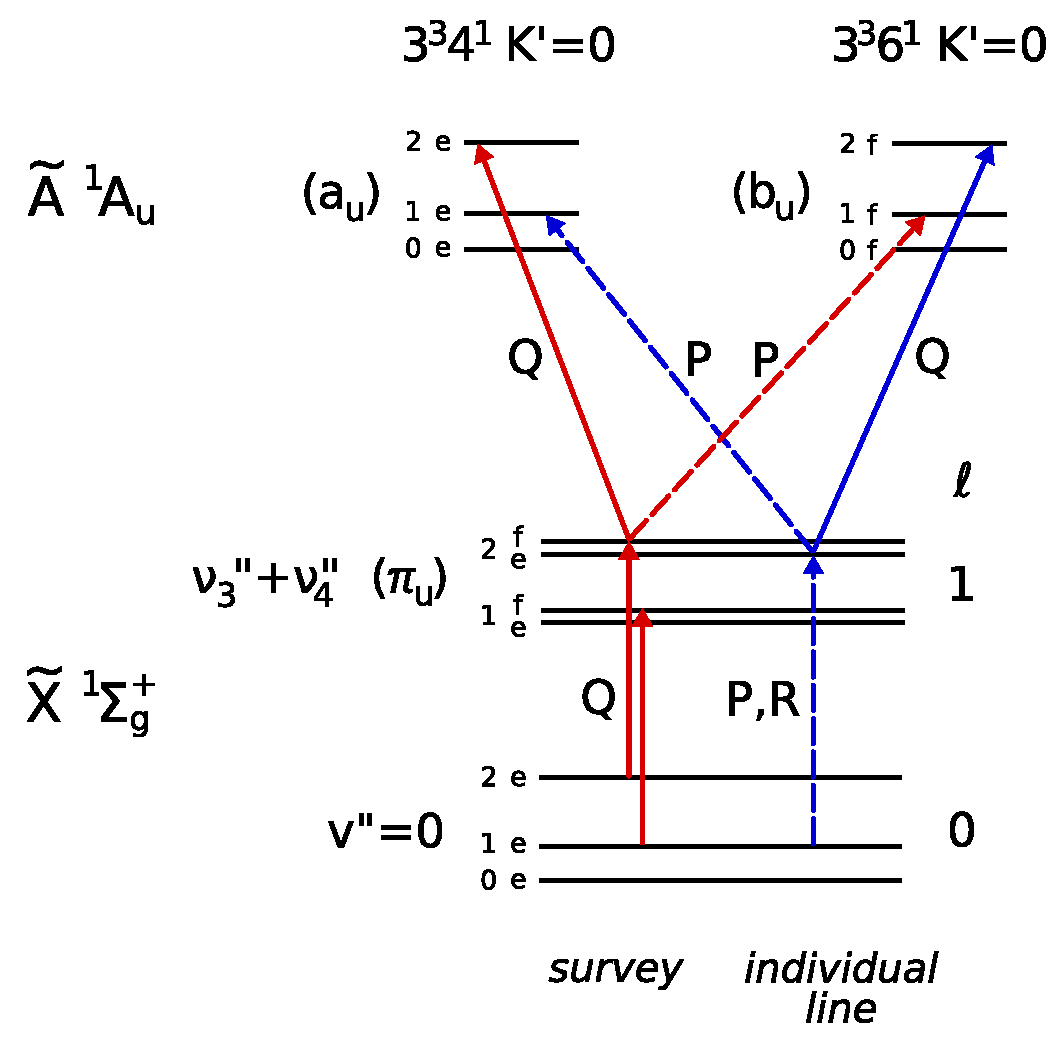
\includegraphics[width=6.2in]{levels-iruvdr}
\end{figure}


\POINT{Say what intermediate states were used for double resonance.}
To collect survey spectra of the $3^36^1$ and $3^34^1$ \Ka{0}
sublevels, the $J=1f-5f$ levels of \xstate\ $\nu_3+\nu_4$
%3897.16 \rcm
were used as intermediate states.  The Q-branch of this band is very
compact, and the incoherent linewidth of the IR laser is sufficient to
excite $J=1f-5f$ at a single laser frequency.

\POINT{Laser resolution $\approx$ 0.094 \rcm; laser step size
  $\approx$ 0.047 \rcm }

\POINT{Describe polarization method used to record the $J'=0$
  spectrum.  (See p.11 in 4/2007--8/2007 notebook.}

\section{Theory: vibrational selection rules for spin-orbit coupling}

\POINT{Discuss spin-orbit selection rules for $\Delta K$, and
  reference tables.}  Spin-orbit selection rules for $N$ and $K$ in
polyatomic molecules are given by Stevens and Brand, and have been
reformulated by other authors \cite{stevens73, howard78, dupre84}.
These follow a subset of the general rules for singlet$\sim$triplet
transitions in polyatomic molecules originally discussed by Hougen
\cite{hougen64}.



\TODO{Show character tables and axis labels for \emph{trans}
  acetylene.  Discuss the correspondence between the ($a,b,c$) axis
  system and the ($x,y,z$).  See p.9, 18--19 in 4/2007--8/2007 notebook.}

\begin{table}
  \centering

  \begin{tabular}{llllrl}
    Vib.
    & $^{v}\Gamma_S$ & $^{ev}\Gamma_S$ & $\Gamma_\sigma$ & $\Delta K$ & $^{v}\Gamma_T$ \\
    \toprule

    $3^3 4^1$ 
    & $a$ & $^{1}A$ & $B$ & $0$ & \textcolor{red}{$a$} \\
    & & & $A, B$ & $\pm1$ & $a, b$ \\[10pt]

    $3^3 6^1$ 
    & $b$ & $^{1}B$ & $B$ & $0$ & \textcolor{red}{$b$} \\
    & & & $A, B$ & $\pm1$ & $a, b$ \\

  \end{tabular}\\[5mm]

  $C_{2}$ symmetry, $^{e}\Gamma_T =$ $^{3}B$
\end{table}

\begin{figure}
  \caption{Rotational factors of spin-orbit matrix elements between
    rovibrational levels of the $S_1$ and $T_3$ electronic states,
    $K_S$=0.  The plot includes all nonzero matrix elements for each
    spin component of a $T_3$ sublevel with $K_T=0,1$.  Transitions
    having $\Delta K = \Delta N = 0$ are forbidden according to
    parity.}
  \centering
  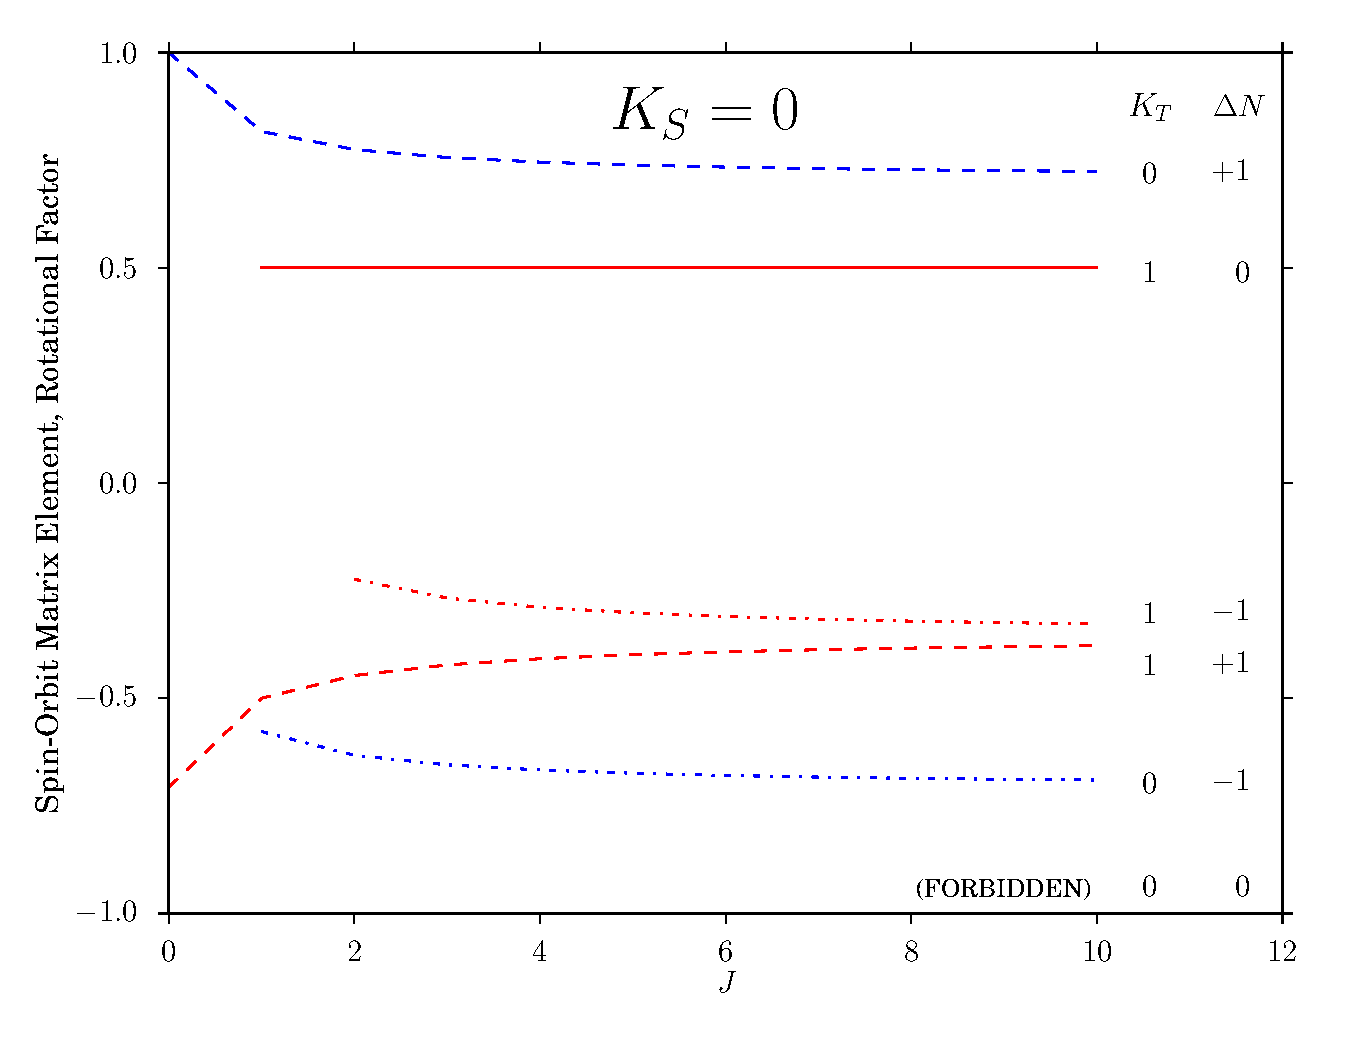
\includegraphics[width=6in]{rotational-factors-k0.pdf}
\end{figure}

Because the $3^34^1$ and $3^36^1$ \Ka{0} sublevels are of opposite
parity, they may not mix with the same triplet sublevels having
$K_T=0$.


\begin{figure}
  \caption{Nonzero matrix elements between the $S_1$ $3^34^1$,
    $3^36^1$ \Ka{0} sublevels and $T_3$ sublevels having $K_T=0$.}
  \label{fig:levels-k0}
  \centering

  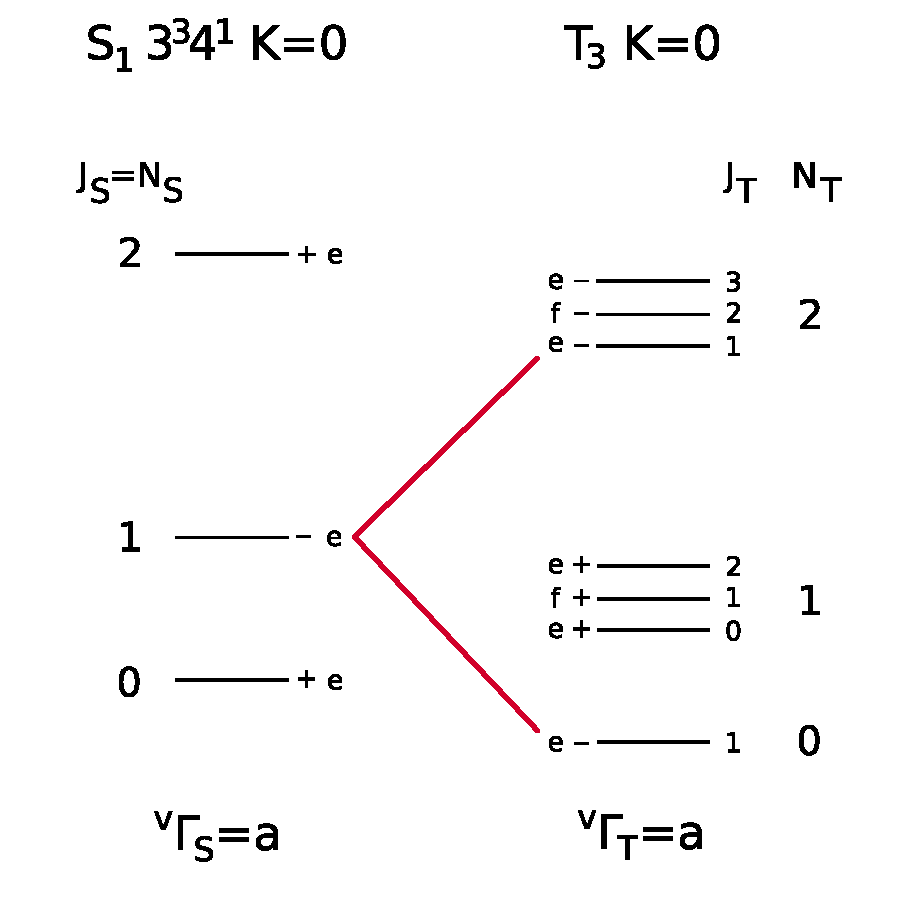
\includegraphics[width=4.2in,angle=90]{levels-3341}
  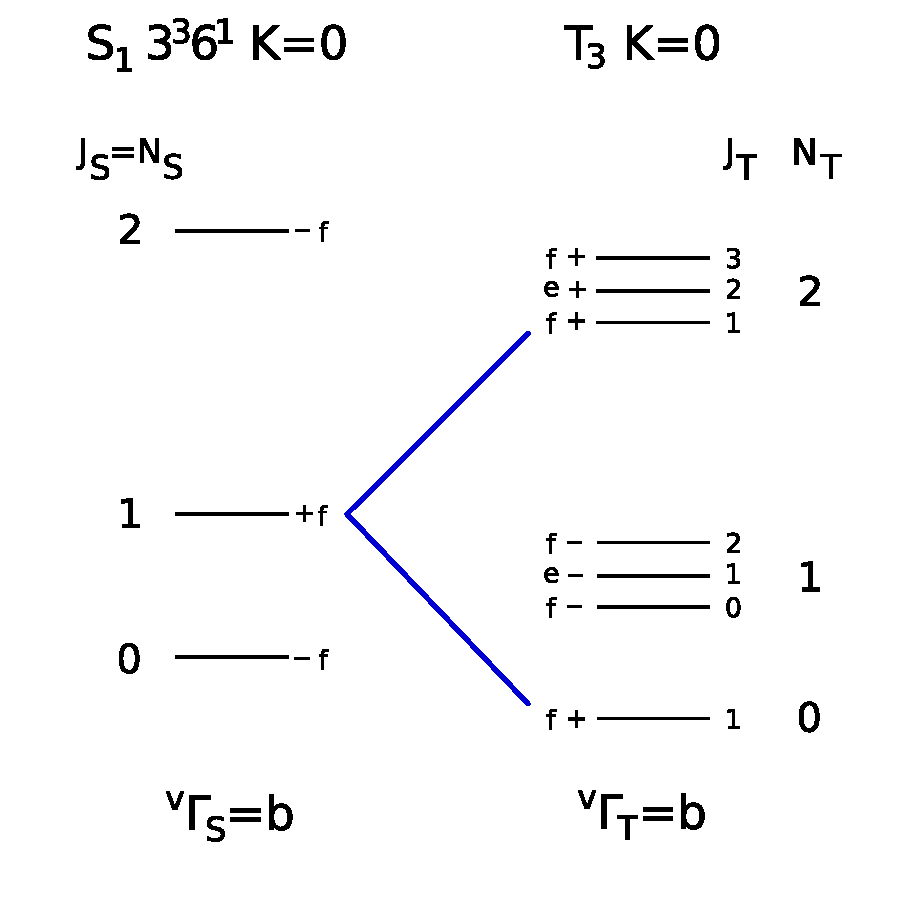
\includegraphics[width=4.2in,angle=90]{levels-3361}  
\end{figure}

\begin{figure}
  \caption{Nonzero matrix elements between the $S_1$ $3^34^1$,
    $3^36^1$ \Ka{0} sublevels and $T_3$ sublevels having $K_T=1$.}
  \label{fig:levels-k1}
  \centering

  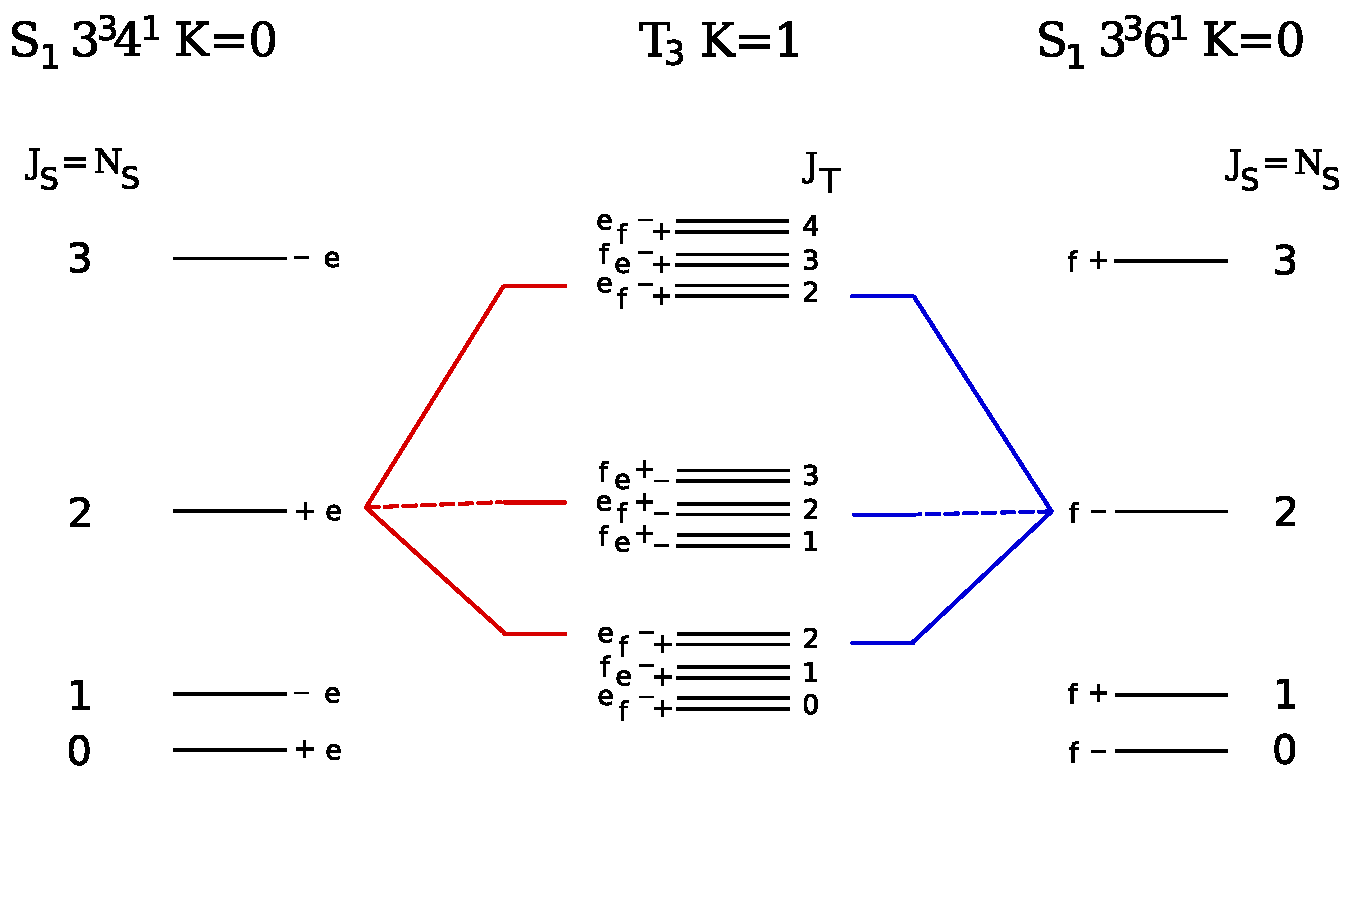
\includegraphics[width=8in,angle=90]{levels-k1}
\end{figure}




\TODO{Use Bryan's program to compute overlap integrals for the two bands.}

\TODO{Show number of modes available in each symmetry as a function
  of energy.}




\section{Results}

%%%%%%%%%%%%%%%%%%%%%%%%%%%%%%%%%%%%%%%%%%%%%%%%%%%%%%
%%
%% INSERT 3^3 6^1 SURVEY FIGURE HERE
%%
%%%%%%%%%%%%%%%%%%%%%%%%%%%%%%%%%%%%%%%%%%%%%%%%%%%%%%

\begin{figure}
  \caption{Simultaneously recorded SEELEM (upper trace) and LIF (lower
    trace) spectra of the $3^36^1$ \Ka{0} sublevel of the \astate\
    state of \ce{C2H2}.  The LIF spectrum is integrated in two time
    regions: an early time window ($1\tau_s-10\tau_s$, solid trace)
    and a delayed time window ($10\tau_s-18\tau_s$, dashed trace).
    \TODO{Describe features of spectrum.}}
  \label{fig:survey-3361}
  \centering
  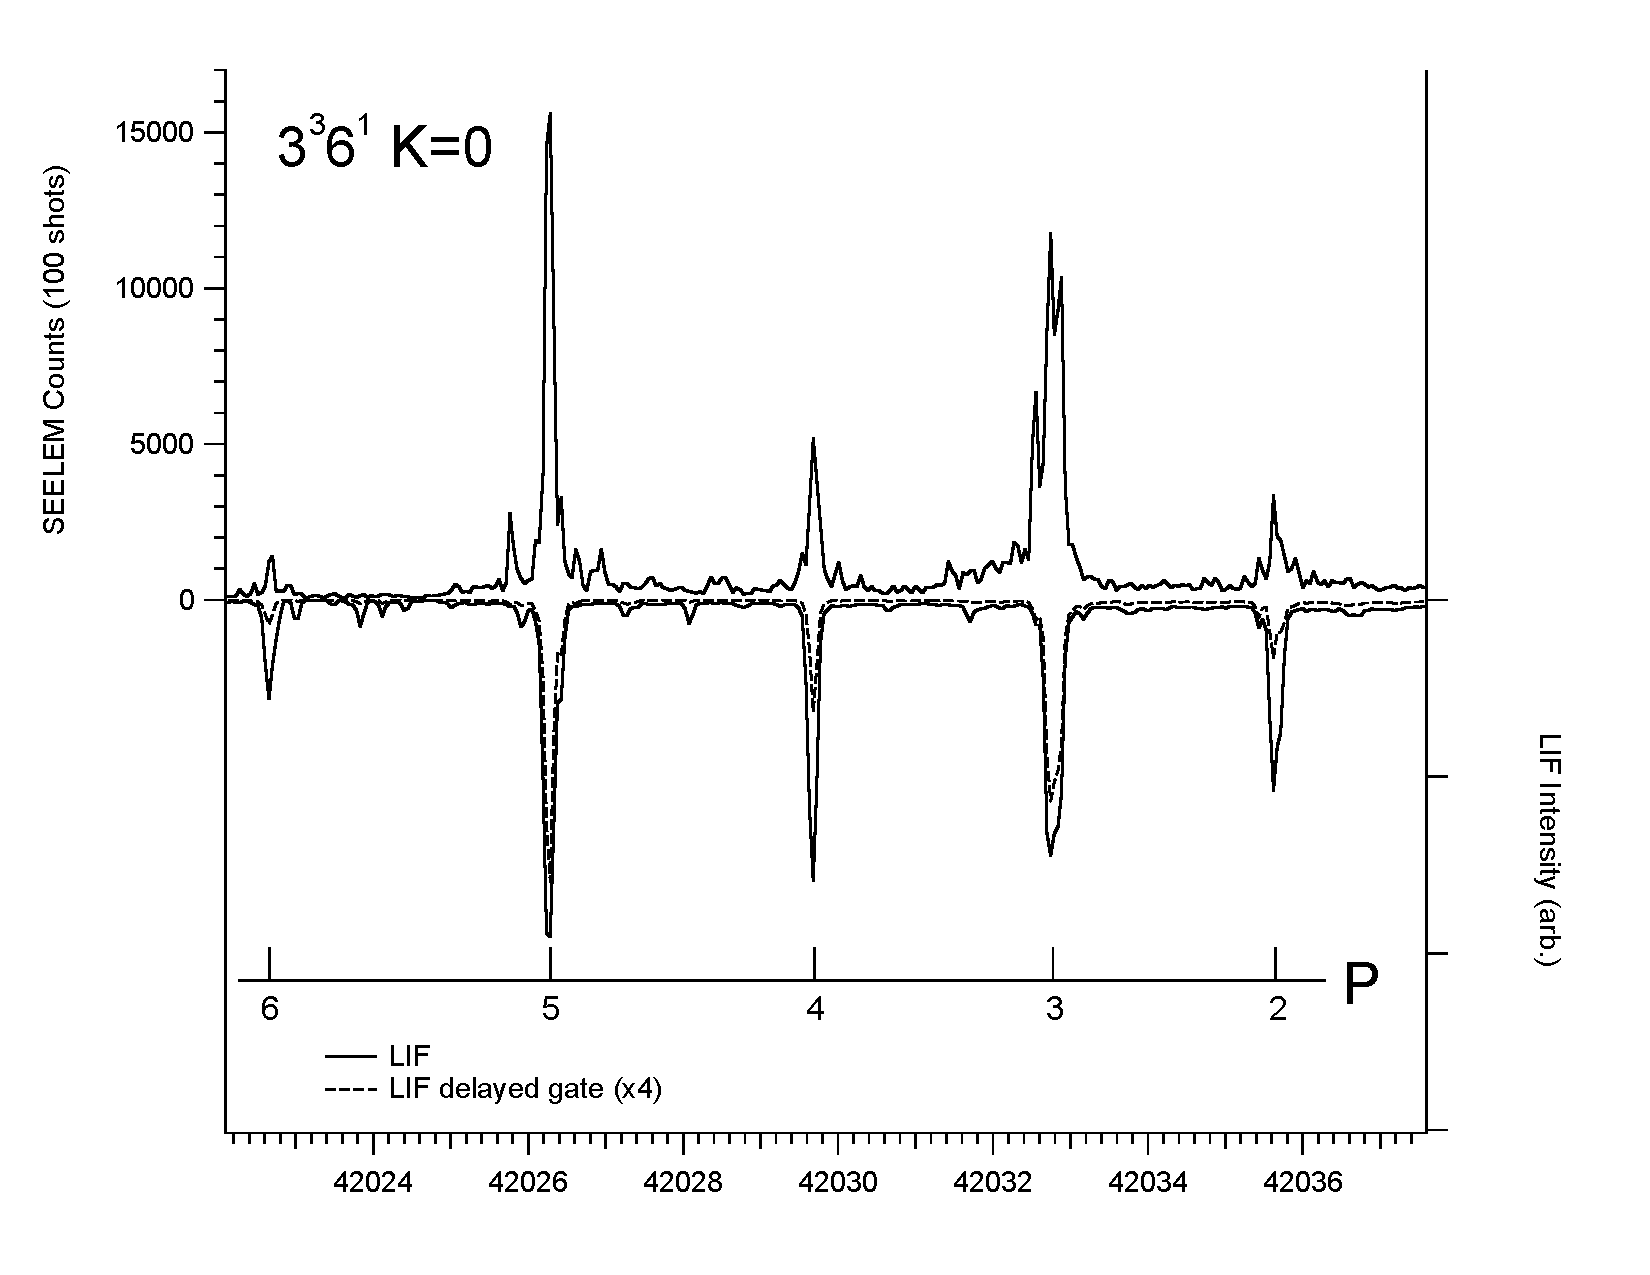
\includegraphics[width=7in,angle=90]{spectrum-3361-p6p2.pdf}
\end{figure}

%%%%%%%%%%%%%%%%%%%%%%%%%%%%%%%%%%%%%%%%%%%%%%%%%%%%%%
%%
%% END 3^3 6^1 SURVEY FIGURE
%%
%%%%%%%%%%%%%%%%%%%%%%%%%%%%%%%%%%%%%%%%%%%%%%%%%%%%%%

The simultaneously recorded SEELEM (plotted upward) and LIF (plotted
downward) spectra of the $3^36^1$ \Ka{1} sublevel of the \astate\
electronic state of acetylene is shown in Figure
\ref{fig:survey-3361}.  This spectrum was recorded by tuning the
infrared laser into resonance with the Q(1-5) rotational lines of the
$3^14^1 \leftarrow 0_0$ ($\Pi - \Sigma$) transition in the ground
state.  Because the Q-branch transitions are very near in frequency,
the $J=1-5$ rotational levels of the intermediate state may be excited
incoherently by tuning the infrared laser to the head of the Q-branch.

%%%%%%%%%%%%%%%%%%%%%%%%%%%%%%%%%%%%%%%%%%%%%%%%%%%%%%
%%
%% INSERT 3^3 6^1 INDIV FIGURES HERE
%%
%%%%%%%%%%%%%%%%%%%%%%%%%%%%%%%%%%%%%%%%%%%%%%%%%%%%%%

\begin{figure}
  \caption{Simultaneously recorded SEELEM (upper trace) and LIF (lower
    trace) spectra of the $3^36^1$ \Ka{0} sublevel of the \astate\
    state of \ce{C2H2}.  The LIF spectrum is integrated in two time
    regions: an early time window ($0.5\tau_s-2\tau_s$, solid trace)
    and a delayed time window ($10\tau_s-18\tau_s$, dashed trace).
    \TODO{Describe features of spectrum.}}
  \label{fig:3361-q1}
  \centering
  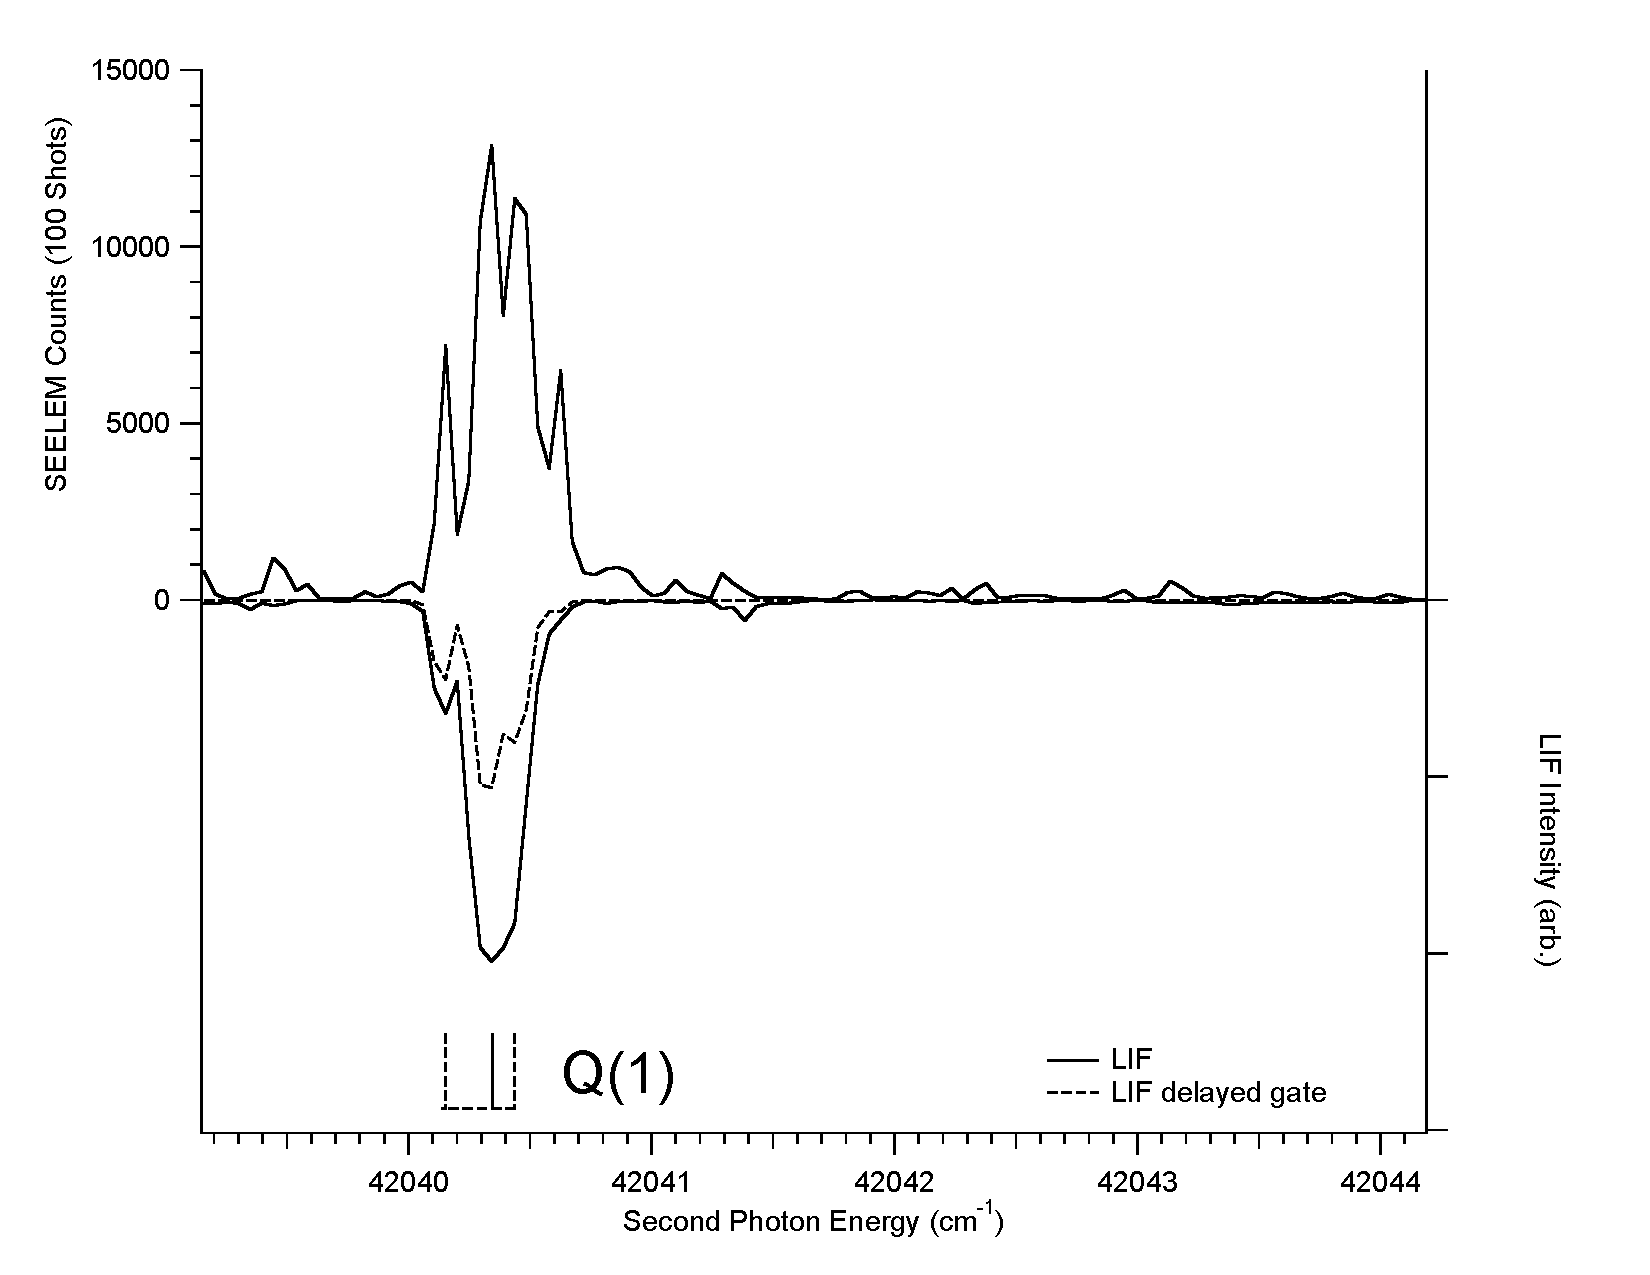
\includegraphics[width=6in]{spectrum-3361-q1-split.pdf}
\end{figure}

\begin{figure}
  \caption{Simultaneously recorded SEELEM (upper trace) and LIF (lower
    trace) spectra of the $3^36^1$ \Ka{0} sublevel of the \astate\
    state of \ce{C2H2}.  The LIF spectrum is integrated in two time
    regions: an early time window ($0.5\tau_s-2\tau_s$, solid trace)
    and a delayed time window ($10\tau_s-18\tau_s$, dashed trace).
    \TODO{Describe features of spectrum.}}
  \label{fig:3361-q2}
  \centering
  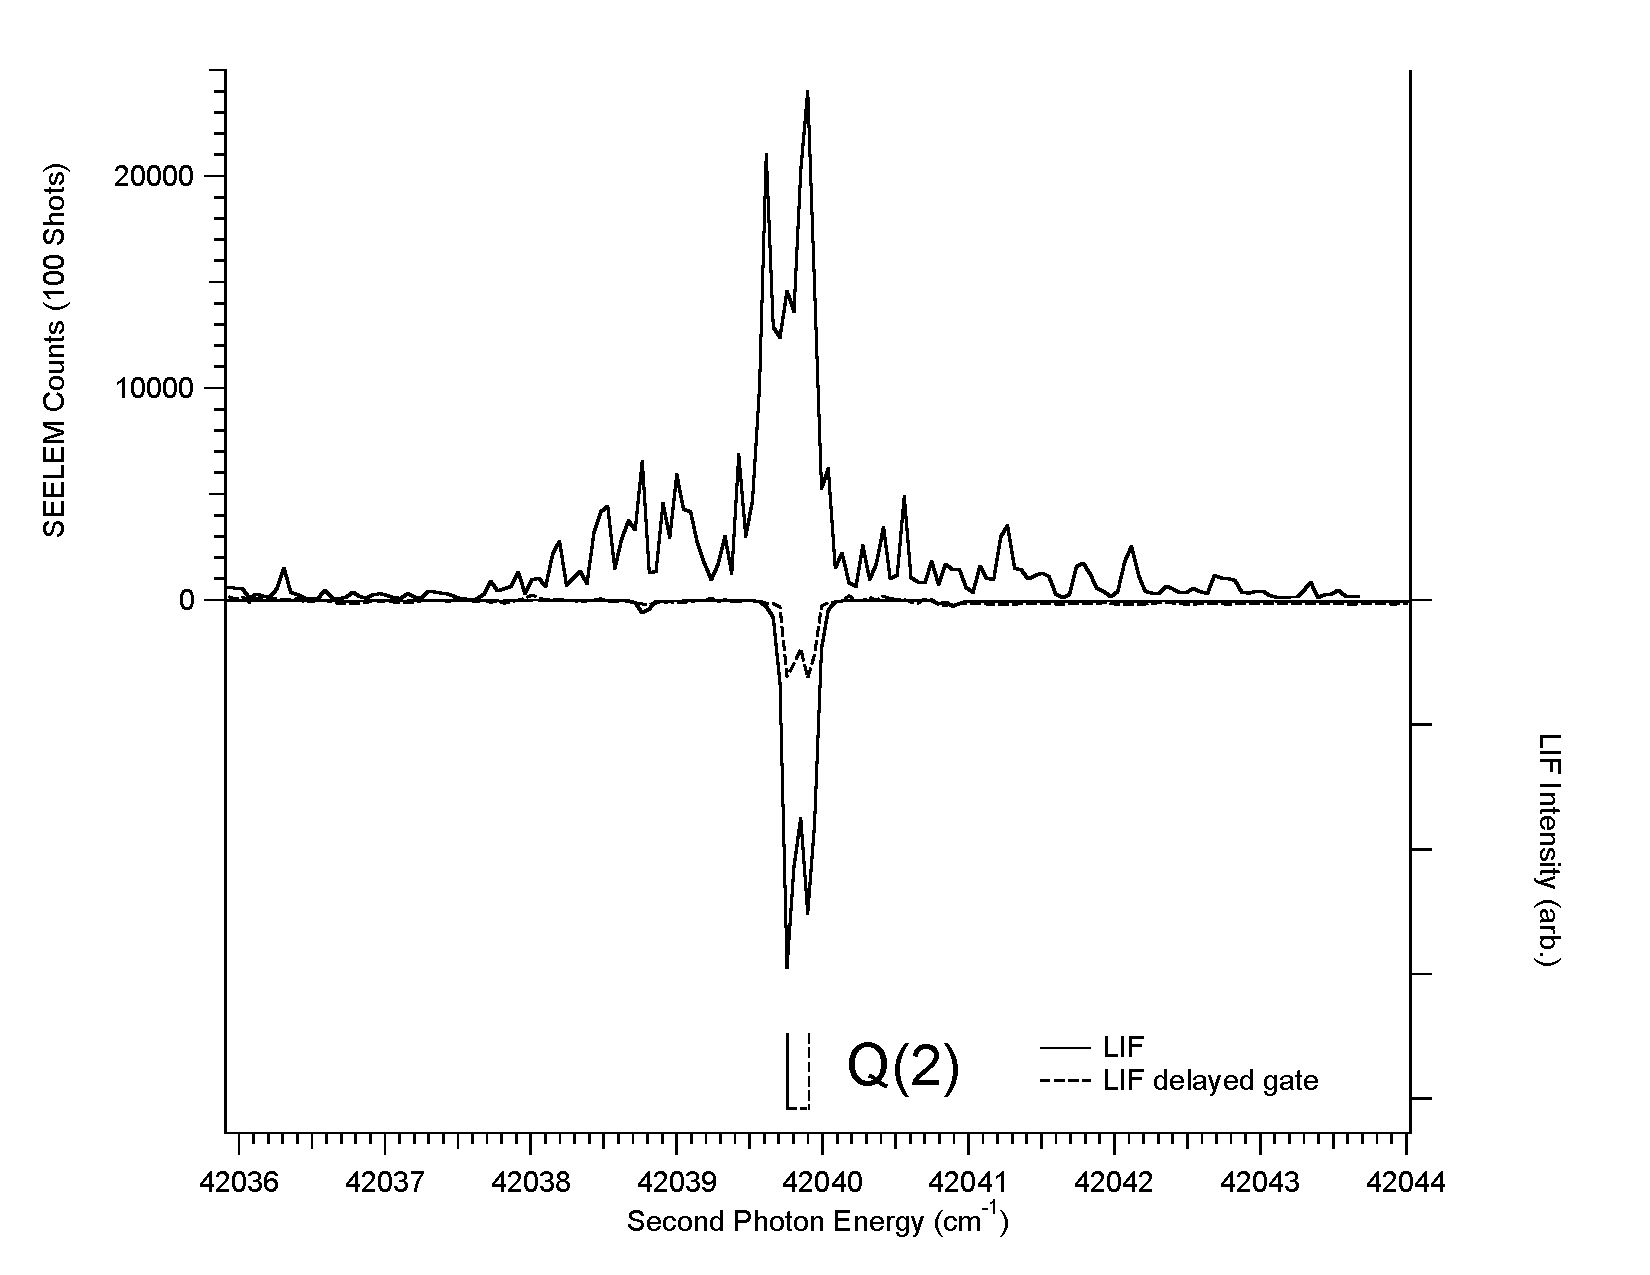
\includegraphics[width=6in]{spectrum-3361-q2-split.pdf}
\end{figure}

\begin{figure}
  \caption{Simultaneously recorded SEELEM (upper trace) and LIF (lower
    trace) spectra of the $3^36^1$ \Ka{0} sublevel of the \astate\
    state of \ce{C2H2}.  The LIF spectrum is integrated in two time
    regions: an early time window ($0.5\tau_s-2\tau_s$, solid trace)
    and a delayed time window ($10\tau_s-18\tau_s$, dashed trace).
    \TODO{Describe features of spectrum.}}
  \label{fig:3361-q3}
  \centering
  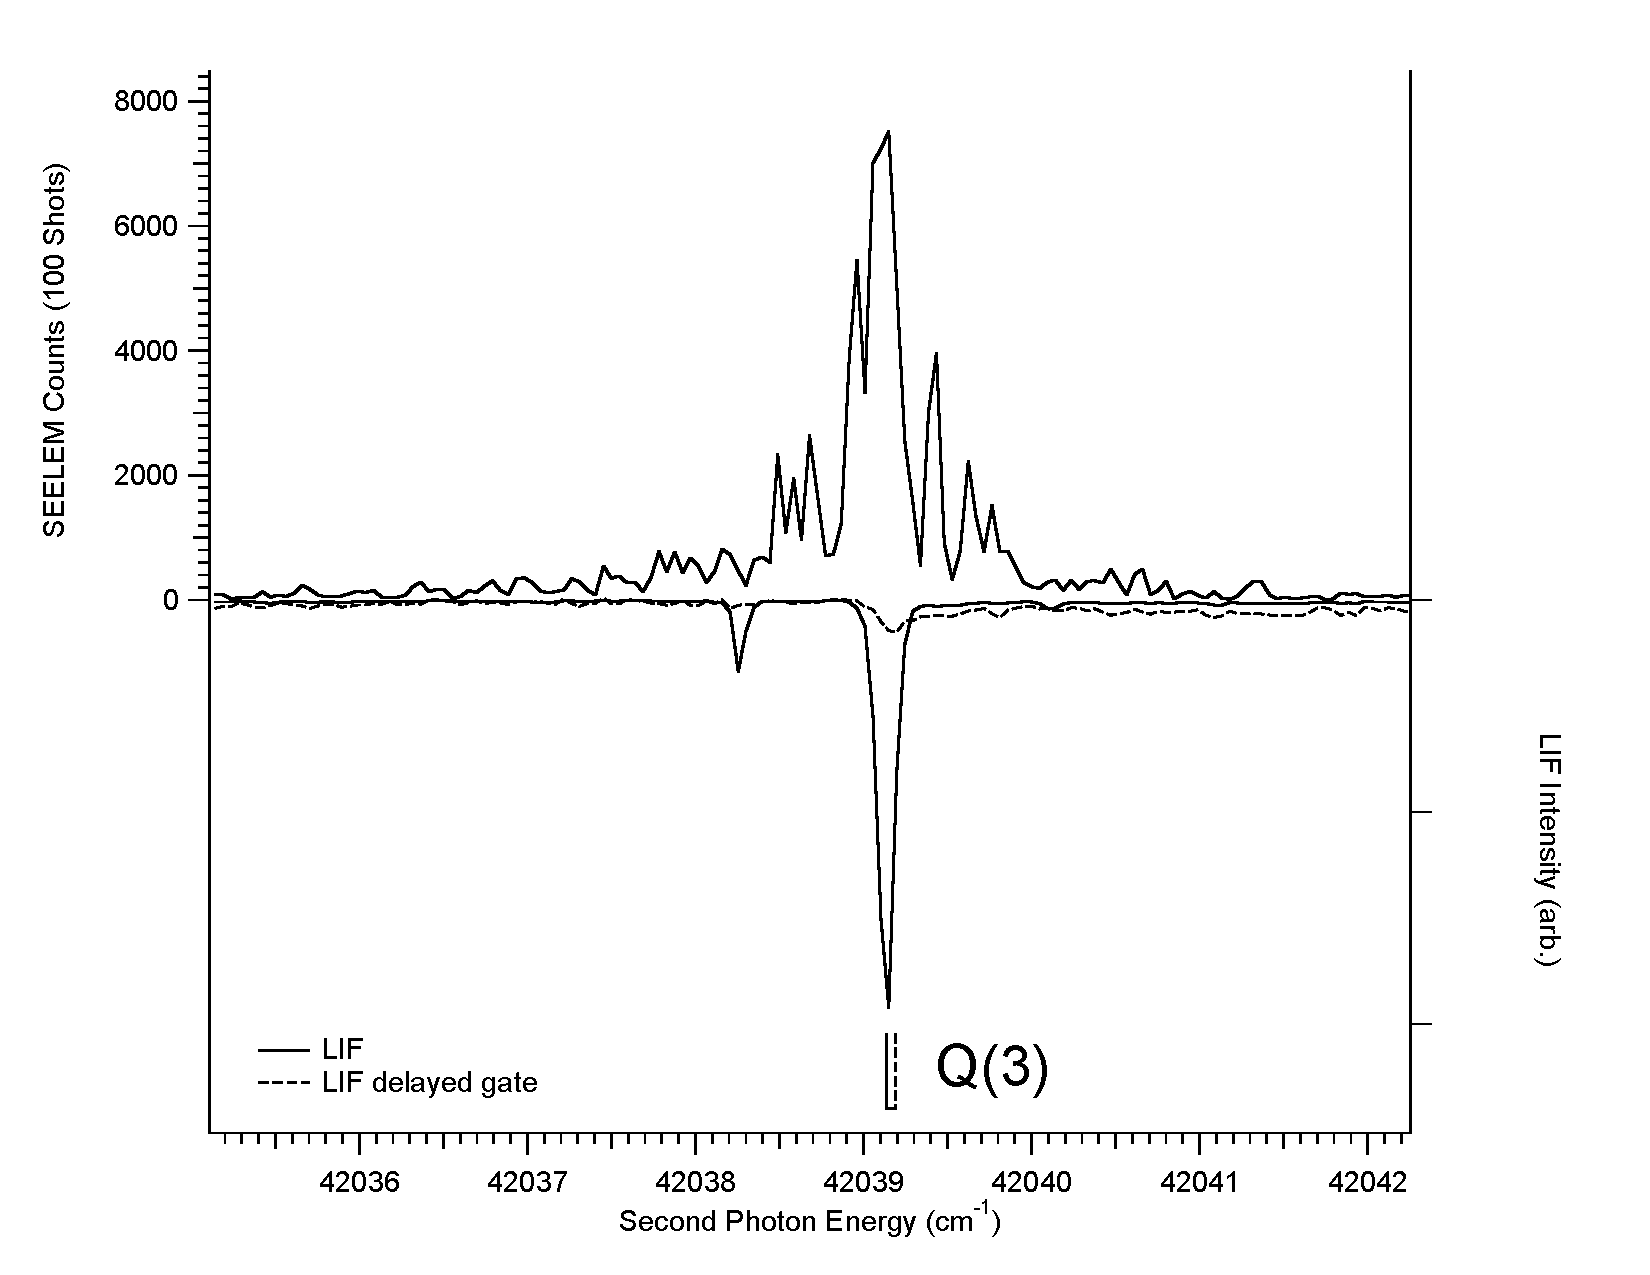
\includegraphics[width=6in]{spectrum-3361-q3-split.pdf}
\end{figure}

\begin{figure}
  \caption{Simultaneously recorded SEELEM (upper trace) and LIF (lower
    trace) spectra of the $3^36^1$ \Ka{0} sublevel of the \astate\
    state of \ce{C2H2}.  The LIF spectrum is integrated in two time
    regions: an early time window ($0.5\tau_s-2\tau_s$, solid trace)
    and a delayed time window ($10\tau_s-18\tau_s$, dashed trace).
    \TODO{Describe features of spectrum.}}
  \label{fig:3361-q4}
  \centering
  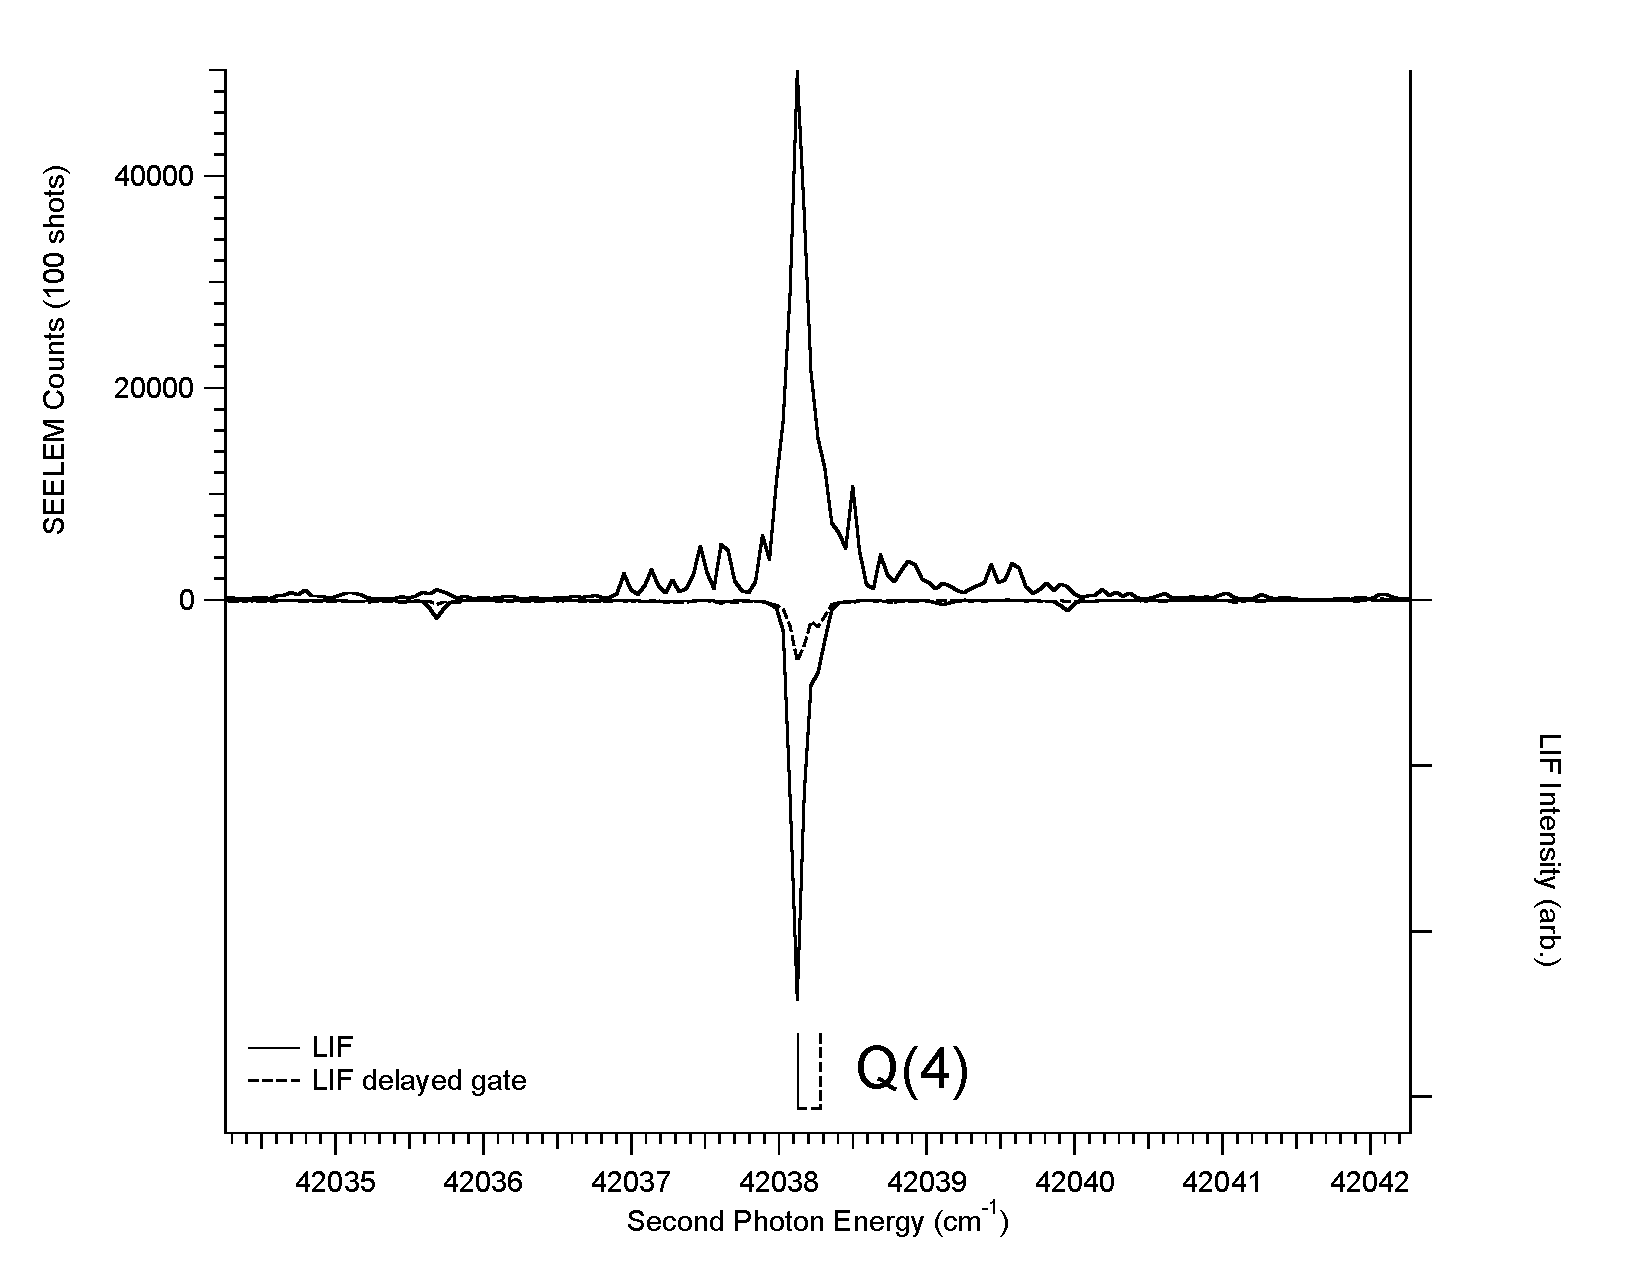
\includegraphics[width=6in]{spectrum-3361-q4-split.pdf}
\end{figure}

\begin{figure}
  \caption{Simultaneously recorded SEELEM (upper trace) and LIF (lower
    trace) spectra of the $3^36^1$ \Ka{0} sublevel of the \astate\
    state of \ce{C2H2}.  The LIF spectrum is integrated in two time
    regions: an early time window ($0.5\tau_s-2\tau_s$, solid trace)
    and a delayed time window ($10\tau_s-18\tau_s$, dashed trace).
    \TODO{Describe features of spectrum.}}
  \label{fig:3361-q5}
  \centering
  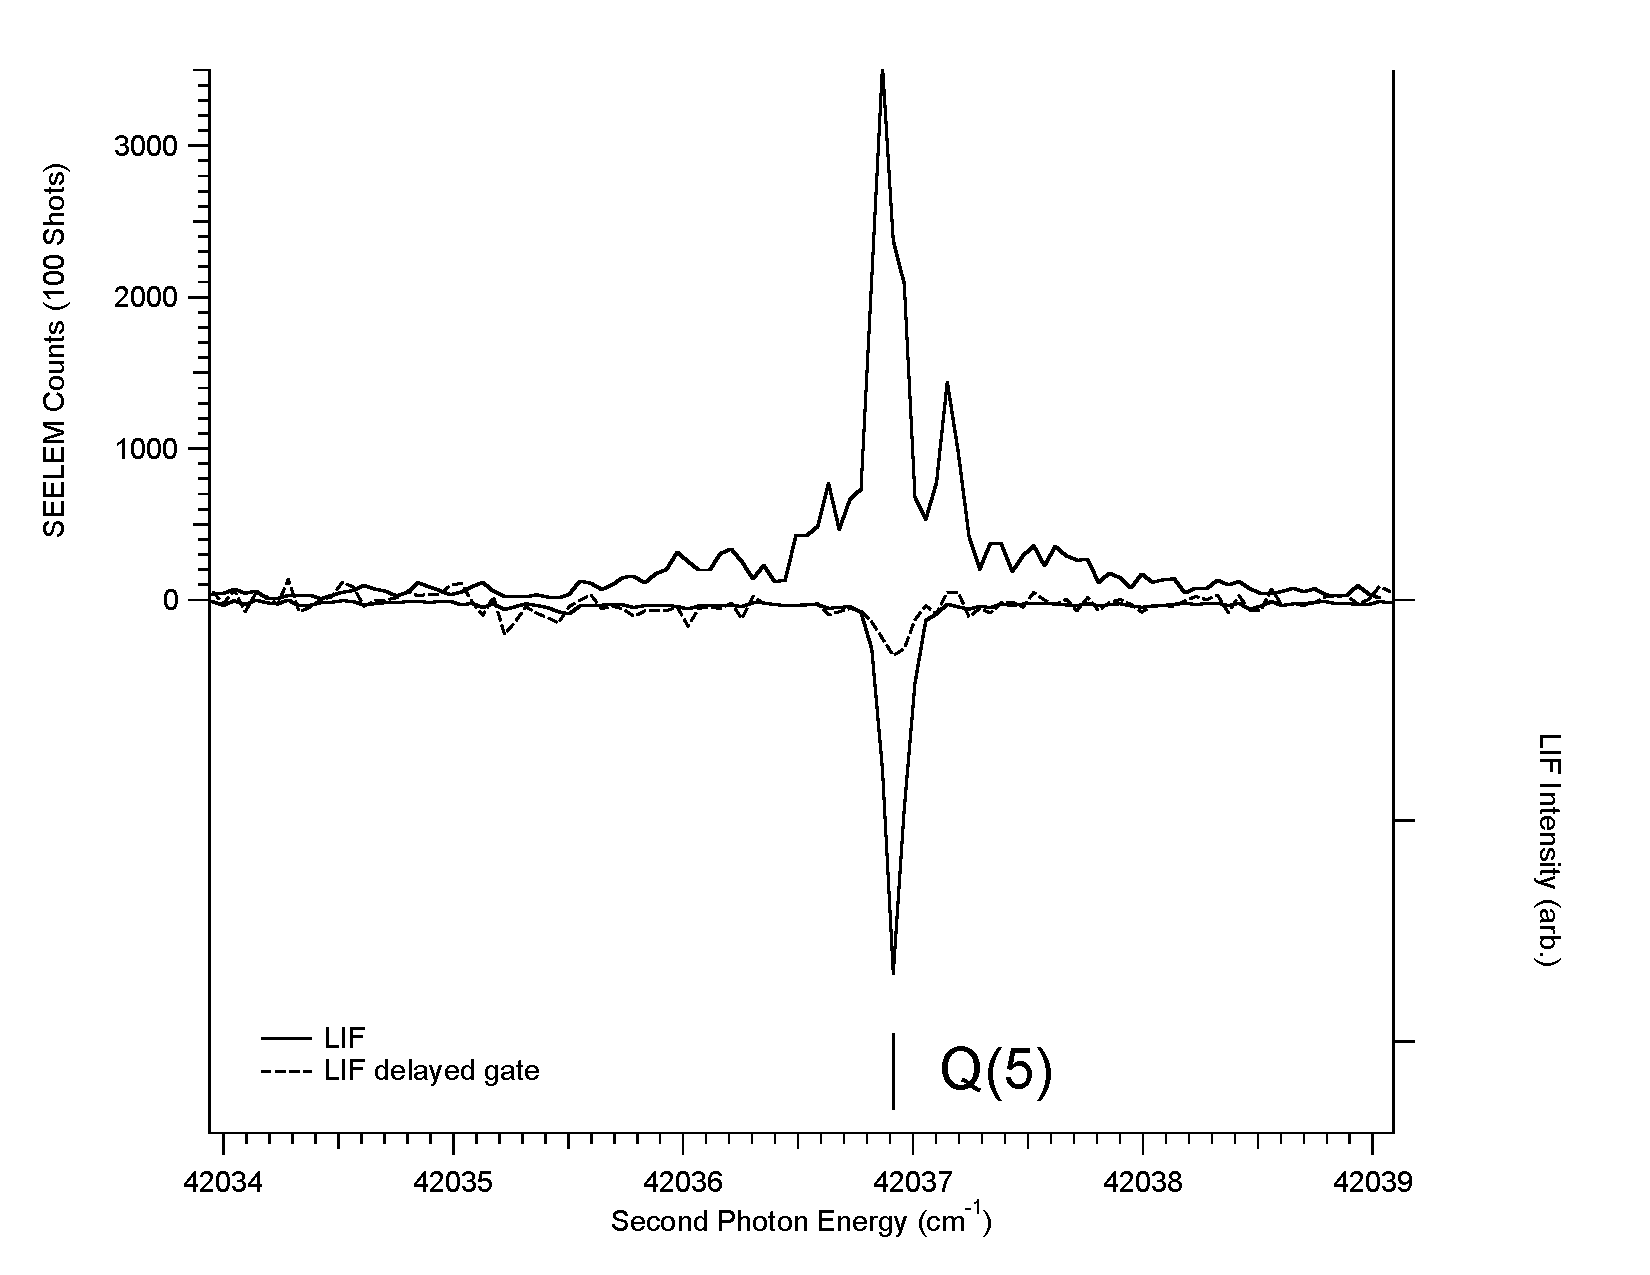
\includegraphics[width=6in]{spectrum-3361-q5-split.pdf}
\end{figure}

%%%%%%%%%%%%%%%%%%%%%%%%%%%%%%%%%%%%%%%%%%%%%%%%%%%%%%
%%
%% END OF 3^3 6^1 INDIV FIGURES
%%
%%%%%%%%%%%%%%%%%%%%%%%%%%%%%%%%%%%%%%%%%%%%%%%%%%%%%%

To observe individual rotational levels in the $3^36^1$ \Ka{0} upper
state, the IR laser was tuned to














\begin{figure}
  \caption{Simultaneously recorded SEELEM (upper trace) and LIF (lower
    trace) spectra of the $3^36^1$ \Ka{0} sublevel of the \astate\
    state of \ce{C2H2}.  The LIF spectrum is integrated in two time
    regions: an early time window ($0.5\tau_s-2\tau_s$, solid trace)
    and a delayed time window ($10\tau_s-18\tau_s$, dashed trace).
    \TODO{Describe features of spectrum.}}
  \label{fig:3361-p1}
  \centering
  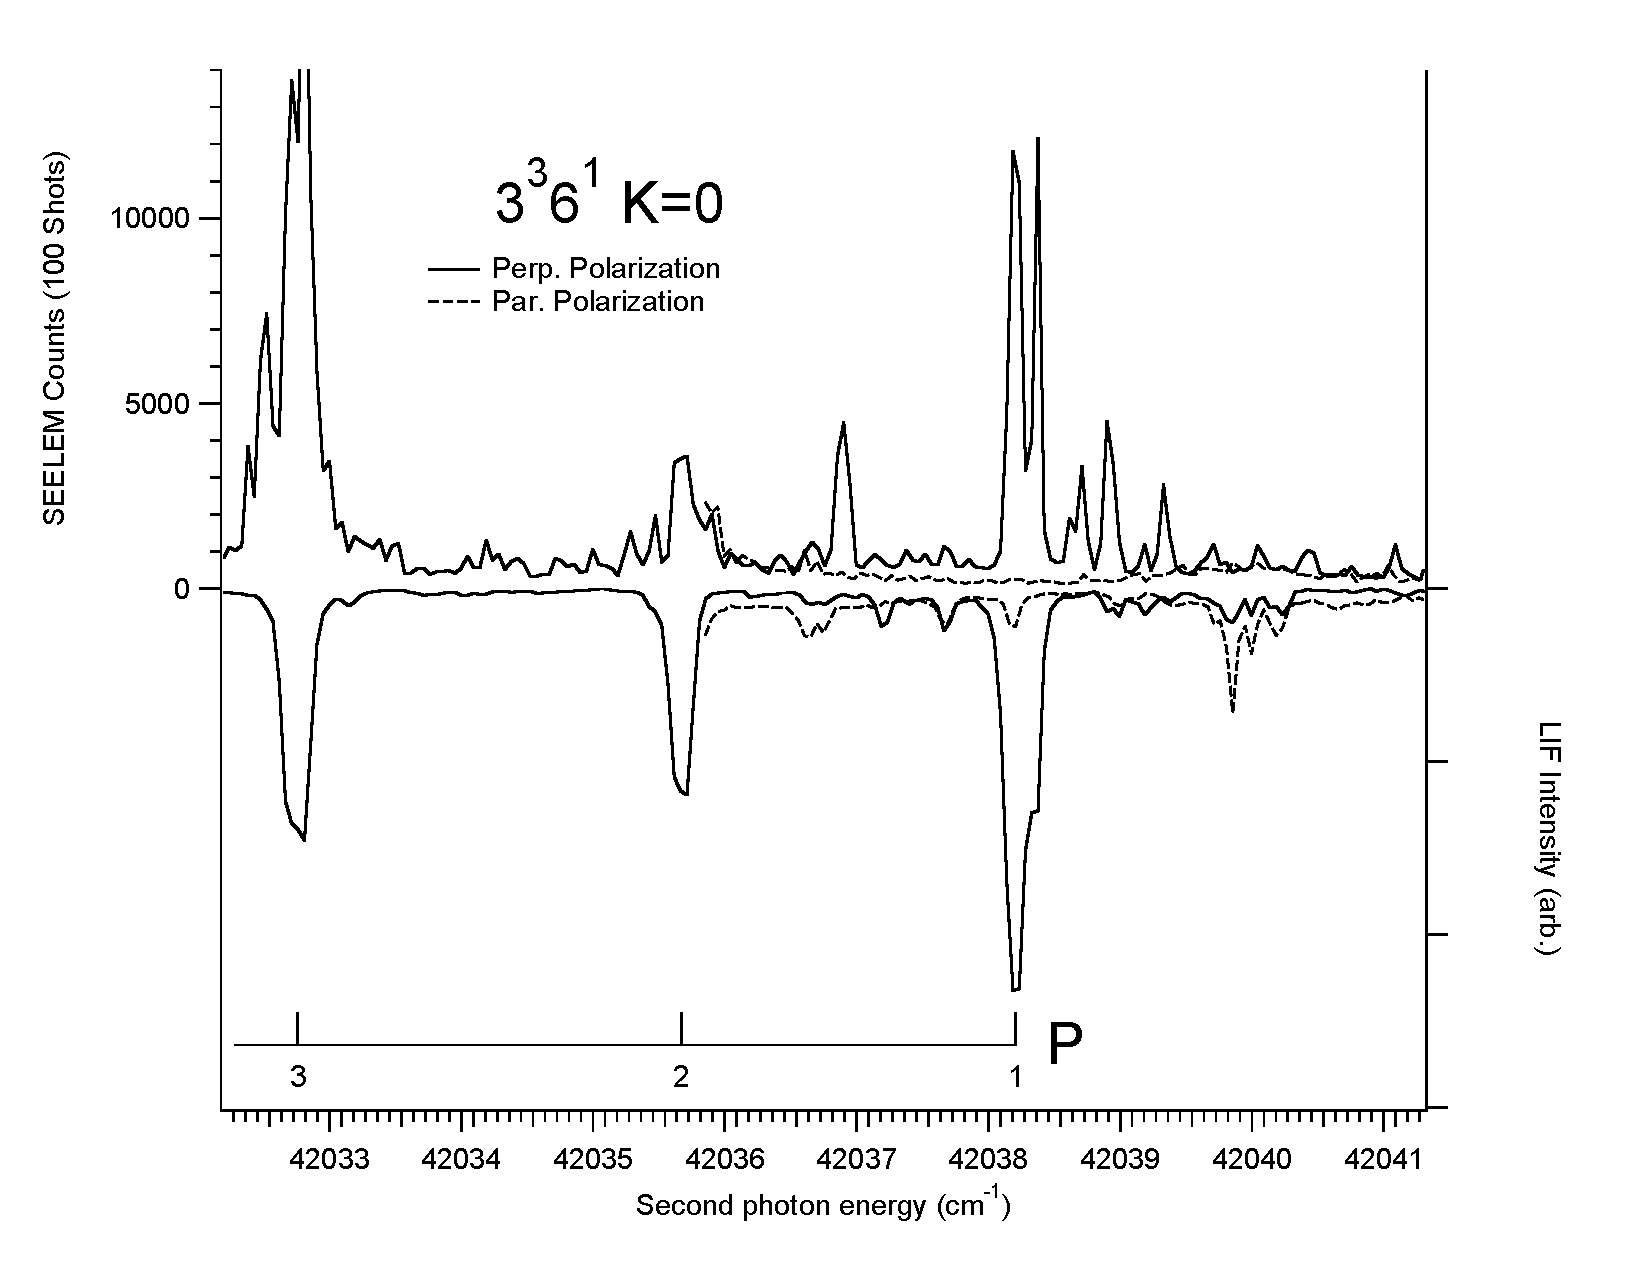
\includegraphics[width=7.3in,angle=90]{spectrum-3361-p1.pdf}
\end{figure}

\begin{figure}
  \caption{Simultaneously recorded SEELEM (upper trace) and LIF (lower
    trace) spectra of the $3^36^1$ \Ka{0} sublevel of the \astate\
    state of \ce{C2H2}.  The LIF spectrum is integrated in two time
    regions: an early time window ($0.5\tau_s-2\tau_s$, solid trace)
    and a delayed time window ($10\tau_s-18\tau_s$, dashed trace).
    \TODO{Describe features of spectrum.}}
  \label{fig:3361-p1}
  \centering
  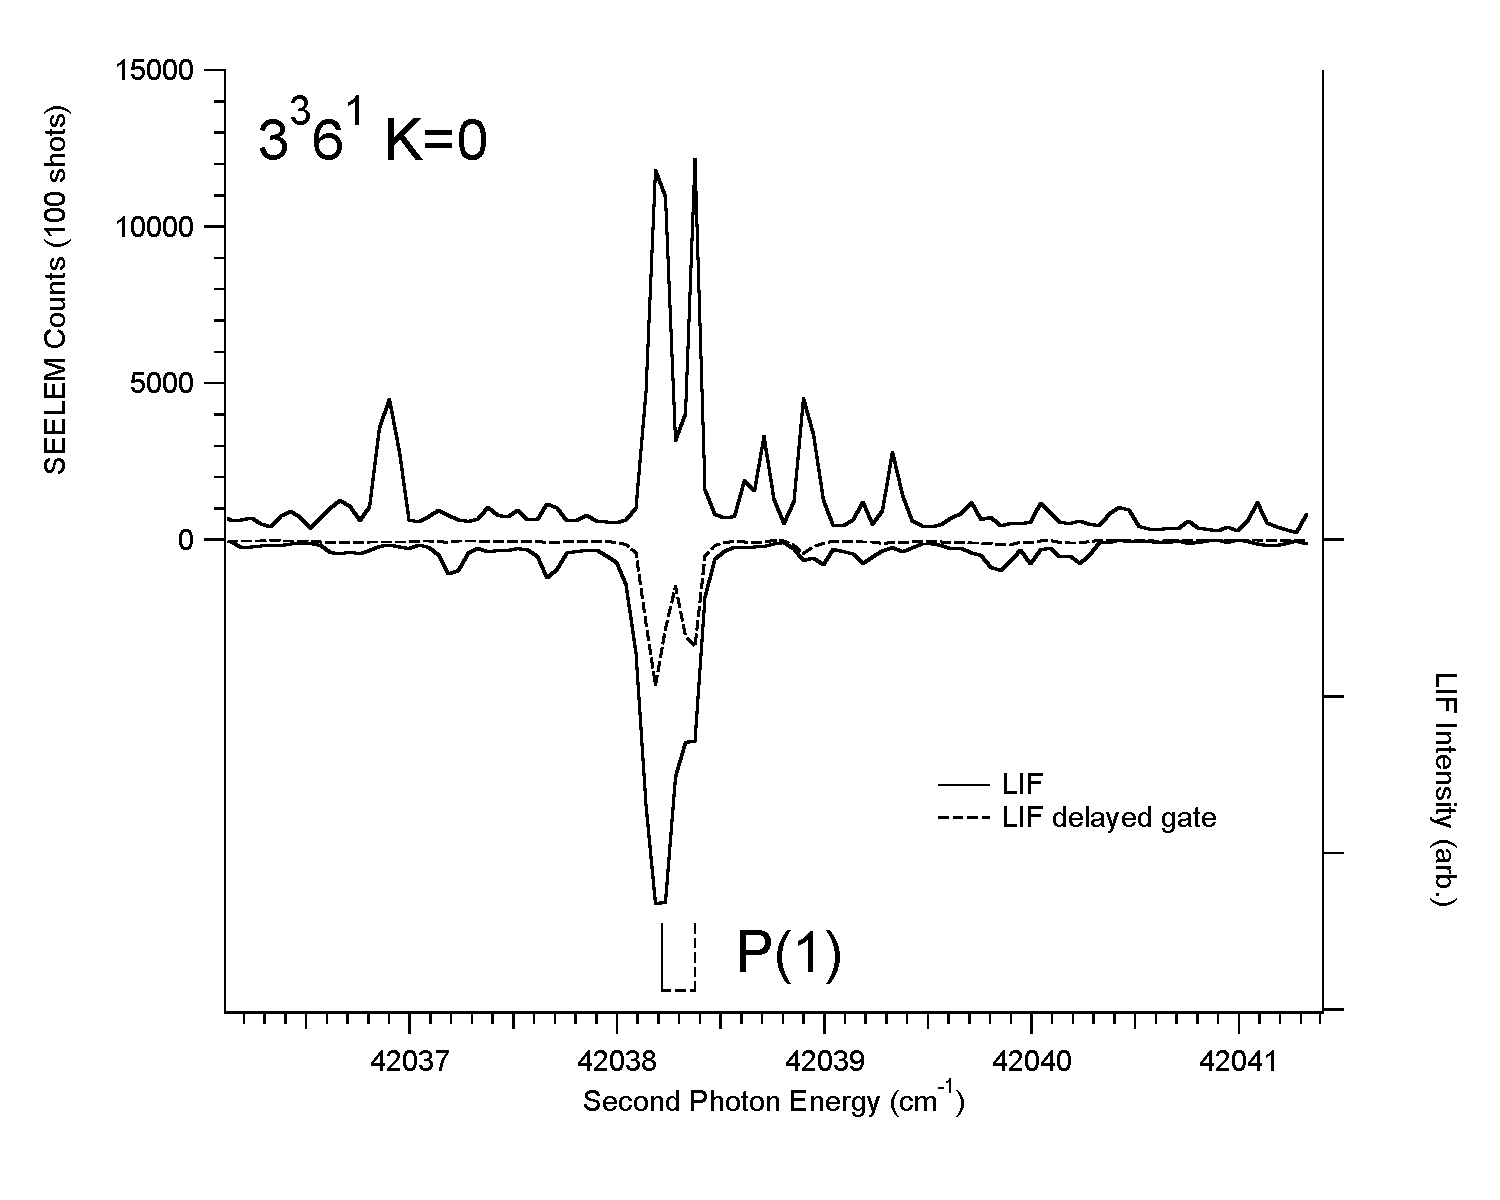
\includegraphics[width=7.3in,angle=90]{spectrum-3361-p1-split.pdf}
\end{figure}

\begin{figure}
  \caption{Simultaneously recorded SEELEM (upper trace) and LIF (lower
    trace) spectra of the $3^34^1$ \Ka{0} sublevel of the \astate\
    state of \ce{C2H2}.  The LIF spectrum is integrated in two time
    regions: an early time window ($1\tau_s-10\tau_s$, solid trace)
    and a delayed time window ($10\tau_s-18\tau_s$, dashed trace).
    \TODO{Describe features of spectrum.}}
  \label{fig:survey-3341}
  \centering
  \includegraphics[width=7in,angle=90]{spectrum-3341-q5q1.pdf}
\end{figure}

\begin{figure}
  \caption{Simultaneously recorded SEELEM (upper trace) and LIF (lower
    trace) spectra of the $3^36^1$ \Ka{0} sublevel of the \astate\
    state of \ce{C2H2}.  The LIF spectrum is integrated in two time
    regions: an early time window ($0.5\tau_s-2\tau_s$, solid trace)
    and a delayed time window ($10\tau_s-18\tau_s$, dashed trace).
    \TODO{Describe features of spectrum.}}
  \label{fig:3341-p2}
  \centering
  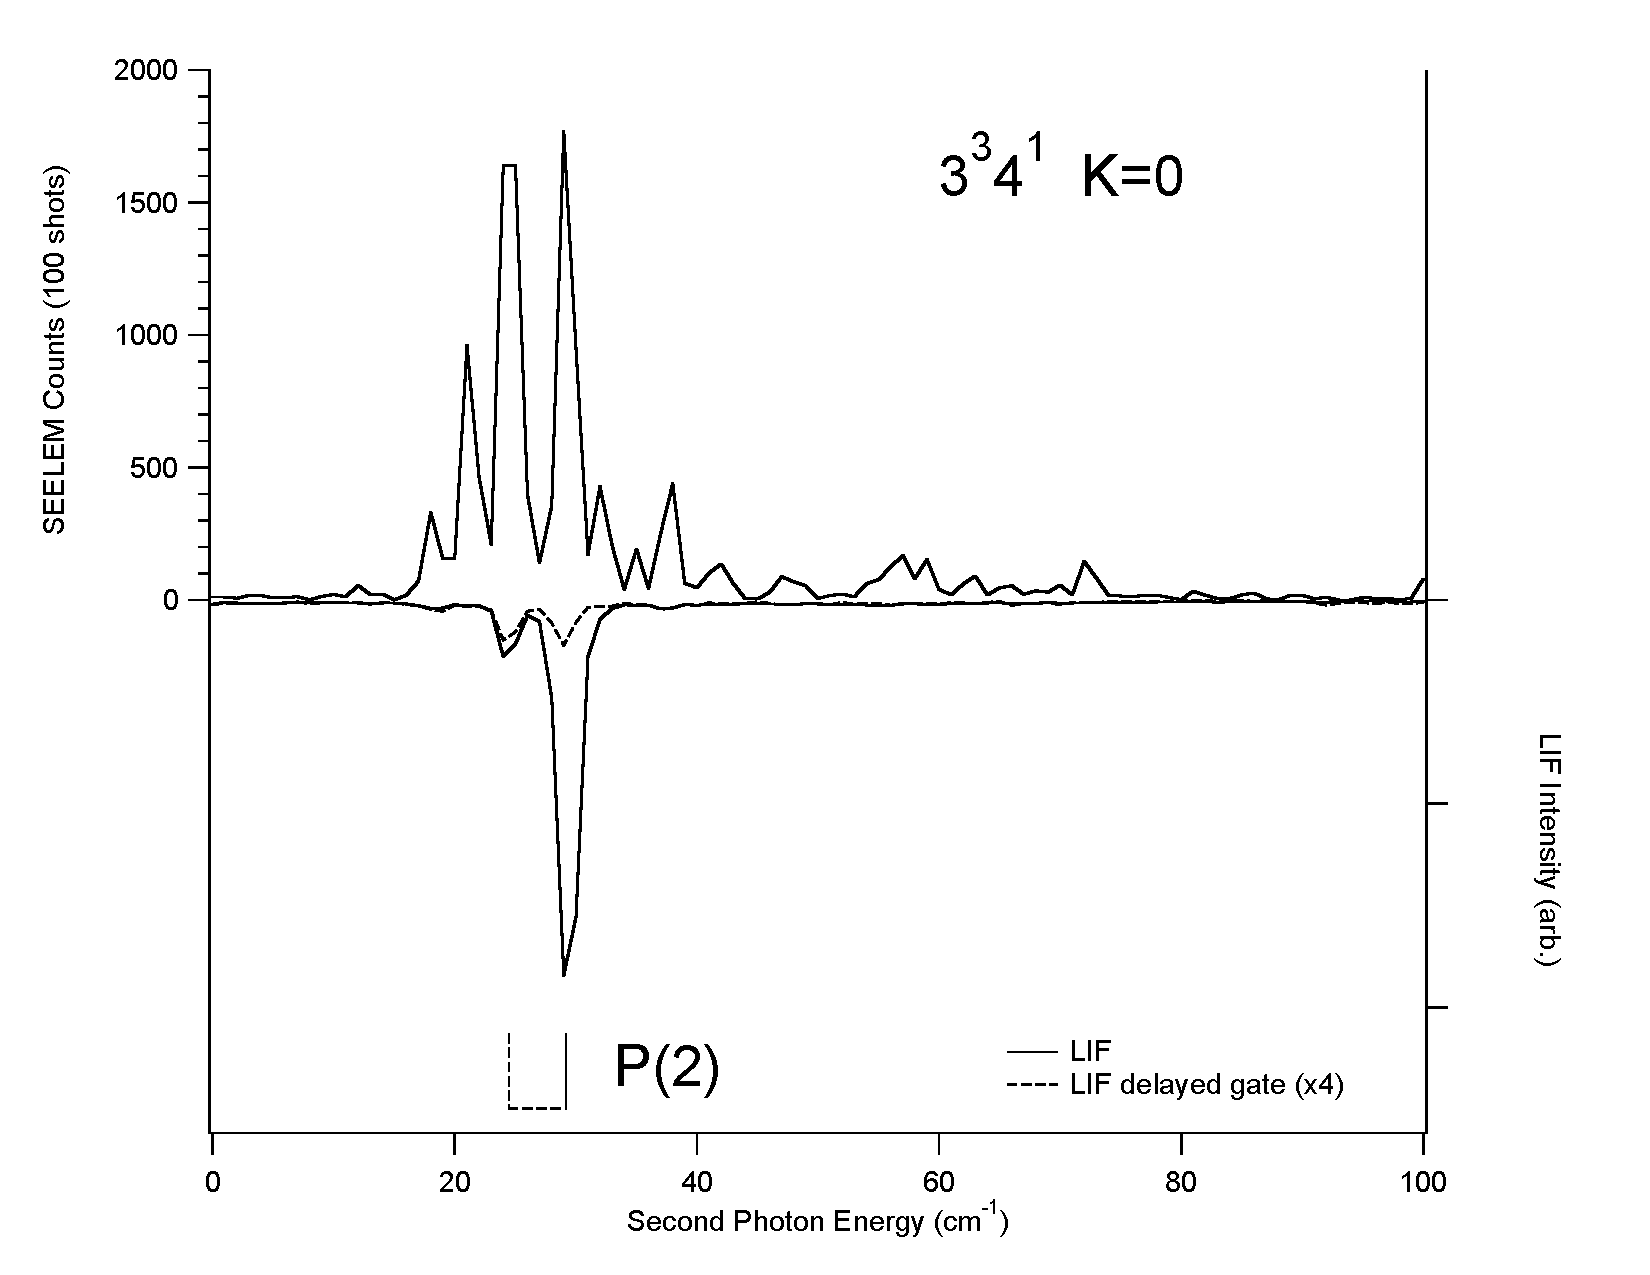
\includegraphics[width=6in]{spectrum-3341-p2-split.pdf}
\end{figure}

\POINT{Present polarization spectrum for rotationless level of
  $3^36^1$.}


\section{Analysis}


\POINT{Present energy levels and reduced term value plot for $3^36^1$.
  (See p.97 of 4/2007--8/2007 notebook.)} 

\POINT{Use $\Delta_3$ statistic, $\Sigma^2$ statistic, or Fourier
  transform methods? (See p.65 in 11/2007--1/2008 notebook.)}

\section{Discussion}

\POINT{Do we see too many doorways, or do we observe what we expect?
  The answer lies in the definition of a doorway state.}

\POINT{The $\nu_3 \sim \nu_6$ anharmonic matrix element is much larger than
  the $\nu_3 \sim \nu_4$ matrix element, and provides a pathway for
  $T_{2,1} \leftarrow T_3 \leftarrow \S_1$ coupling.}

\section{Conclusion}

\section{Recycle bin}

\emph{This spring, Adam and Hans were mapping out the non-symmetric
  bending polyads of acetylene in IR-UV double resonance experiments.
  During this process, they encountered a number of vibrational
  subbands with telltale signs of singlet-triplet coupling: long
  lifetimes, fractionation, and strong quantum beats.  With help from
  Hans, Wilton and I were able to study a few of these bands with the
  SEELEM detector, illuminating the metastable eigenstates connected
  to these allowed transitions.}


Several recent \emph{ab initio} calculations have established a
non-planar equilibrium geometry for the $T_3$ state of acetylene.  The
most recent claculations by Bryan Wong [\emph{JCP} 126, 184307 (2007)]
give a torsional angle of $105^\circ$, which is well in line with the
earlier results of Ventura \emph{et al} [\emph{JCP} 118, 1702 (2003)].
Since the $T_3$ state is known to play a role in coupling the $S_1$
state to the bath of metastable $T_{1,2}$ states, we wish to
investigate vibrational motions that may promote coupling between
$S_1$ and $T_3$.  In particular, we are interested in the torsional
mode $\nu_4'$, which twists the molecule out of a planar geometry.

However, the two non-symmetric bending modes $\nu_4'$ and $\nu_6'$ are
strongly coupled by Darling-Dennison and a-type Coriolis interactions.
Our recent submission to \emph{JPC A} contains an overview of these
effects as they relate to singlet-triplet coupling.  Anthony Merer and
the Singlets understand these couplings very well and are now in the
process of writing what is sure to be the classic paper on this topic.

We wanted to ivestigate subbands where these effects are not present.

both $K=0$ subbands show signs of strong singlet-triplet mixing.

This particular polyad has been studied before. The most relevant
paper is Nami and Soji's study of Zeeman quantum beats in the $3^3 B^1
K=1$ subbands [\emph{CPL} 348, 53 (2001)].  They observe strong
splitting and Zeeman quantum beats in the $3^3 6^1$ band, but not in
the band involving torsion.

Our results follow.  The first two spectra give an overview of both
bands.  We use overlapping transitions of $J'=1-6$ in the Q-branch of
the intermediate state to take spectra that \emph{look} like
one-photon spectra.  Unlike Nami and Soji's observations in the $K=1$
levels, we observe splittings and strong SEELEM signal in the $3^3
4^1$ band when $K=0$.

The major advantage of working in double resonance is of course the
ability to simplify the spectrum.  This is especially beneficial for
SEELEM experiments, because the manifold of metastable states
borrowing intensity from one rotational level often overlaps with that
of the next.  We examined each rotational level in turn for $3^3 6^1$,
collecting SEELEM data for each rotational level of the bright state
without overlap from neighboring levels.  Since the spin-orbit
operator is diagonal in $J$, we get this quantum number for free when
we examine one rotational transition at a time.

The SEELEM signals for these transitions are the strongest we have
ever recorded for acetylene.  Even the ``weak'' intensity regions are
full of well-resolved lines, as illustrated in a close-up of our data
from $J'=4$.

Too top it all off, our choice of $K=0$ bands allowed us to observe
the rotationless level of the bright state, coupled to $J'=0$ and
$K_T=0,1$ levels in the triplet manifold.  In $3^3 6^1$, we couldn't use
a P or R-branch transition in the intermediate state to single out
this level, but we were able to use polarization to record a SEELEM
spectrum without the $J'=0$ levels.

\bibliography{master}
\bibliographystyle{plain}
\end{document}